\usetikzlibrary{arrows.meta}
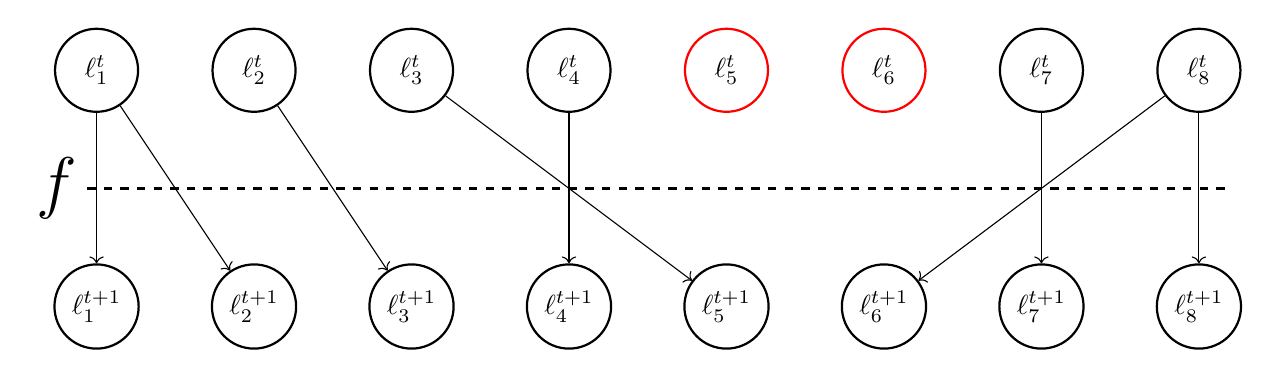
\begin{tikzpicture}
    \begin{scope}[auto, every node/.style={draw=black,circle,thick,minimum size=3em}]
        \node (A_1) at (0, 0) {$\ell^{t+1}_1$};
        \node (A_2) at (2, 0) {$\ell^{t+1}_2$};
        \node (A_3) at (4, 0) {$\ell^{t+1}_3$};
        \node (A_4) at (6, 0) {$\ell^{t+1}_4$};
        \node (A_5) at (8, 0) {$\ell^{t+1}_5$};
        \node (A_6) at (10, 0) {$\ell^{t+1}_6$};
        \node (A_7) at (12, 0) {$\ell^{t+1}_7$};
        \node (A_8) at (14, 0) {$\ell^{t+1}_8$};

        \node (B_1) at (0, 3) {$\ell^{t}_1$};
        \node (B_2) at (2, 3) {$\ell^{t}_2$};
        \node (B_3) at (4, 3) {$\ell^{t}_3$};
        \node (B_4) at (6, 3) {$\ell^{t}_4$};
        \node (B_7) at (12, 3) {$\ell^{t}_7$};
        \node (B_8) at (14, 3) {$\ell^{t}_8$};

        \node[draw=red] (B_5) at (8, 3) {$\ell^{t}_5$};
        \node[draw=red] (B_6) at (10, 3) {$\ell^{t}_6$};
    \end{scope}

    \begin{scope}
        \node (C_1) at (-0.5, 1.5) {\Huge$f$};
        \node (C_2) at (14.5, 1.5) {};
        \draw[thick, dashed] (C_1) -- (C_2);
    \end{scope}

    \begin{scope}[every edge/.style={draw=black}]
        \path[->] (B_1) edge (A_2);
        \path[->] (B_1) edge (A_1);
        \path[->] (B_2) edge (A_3);
        \path[->] (B_3) edge (A_5);
        \path[->] (B_4) edge (A_4);
        \path[->] (B_8) edge (A_6);
        \path[->] (B_8) edge (A_8);
        \path[->] (B_7) edge (A_7);
    \end{scope}
\end{tikzpicture}